\documentclass[conference]{IEEEtran}
\IEEEoverridecommandlockouts
% The preceding line is only needed to identify funding in the first footnote. If that is unneeded, please comment it out.
\usepackage{cite}
\usepackage{amsmath,amssymb,amsfonts}
\usepackage{algorithmic}
\usepackage{graphicx}
\usepackage{textcomp}
\usepackage{xcolor}
\usepackage{multirow}
\usepackage{rotating}
\usepackage{mdframed}
\usepackage{hyperref}
\usepackage{tikz}
\usepackage{makecell}
\usepackage{tcolorbox}
\usepackage{amsthm}
%\usepackage[english]{babel}
\usepackage{pifont} % checkmarks
%\theoremstyle{definition}
%\newtheorem{definition}{Definition}[section]

\usepackage{listings}
\lstset
{ 
    basicstyle=\footnotesize,
    numbers=left,
    stepnumber=1,
    xleftmargin=5.0ex,
}

%SCJ
\usepackage{subcaption}
\usepackage{array, multirow}
\usepackage{enumitem}

\def\BibTeX{{\rm B\kern-.05em{\sc i\kern-.025em b}\kern-.08em
    T\kern-.1667em\lower.7ex\hbox{E}\kern-.125emX}}
\begin{document}

%\IEEEpubid{978-1-6654-8356-8/22/\$31.00 ©2022 IEEE}
% @Sune:
% Found this suggestion: https://site.ieee.org/compel2018/ieee-copyright-notice/
% I have added it - you can see if it fulfills the requirements

%\IEEEoverridecommandlockouts
%\IEEEpubid{\makebox[\columnwidth]{978-1-6654-8356-8/22/\$31.00 ©2022 IEEE %\hfill} \hspace{\columnsep}\makebox[\columnwidth]{ }}
                                 %978-1-6654-8356-8/22/$31.00 ©2022 IEEE
% copyright notice added:
%\makeatletter
%\setlength{\footskip}{20pt} 
%\def\ps@IEEEtitlepagestyle{%
%  \def\@oddfoot{\mycopyrightnotice}%
%  \def\@evenfoot{}%
%}
%\def\mycopyrightnotice{%
%  {\footnotesize 978-1-6654-8356-8/22/\$31.00 ©2022 IEEE\hfill}% <--- Change here
%  \gdef\mycopyrightnotice{}% just in case
%}
      
\title{Software Architecture for a pharmaceutical company \\
}

\author{
    \IEEEauthorblockN{
        Md Al Imran Khan 1\IEEEauthorrefmark{1},
        Nima Moayedzadeh 2\IEEEauthorrefmark{1},
        Peter Balint Jenovari 3\IEEEauthorrefmark{1},
        Md Iqbal Hossain 4\IEEEauthorrefmark{1},
    }
    \IEEEauthorblockA{
        University of Southern Denmark, SDU Software Engineering, Odense, Denmark \\
        Email: \IEEEauthorrefmark{1} \textnormal{\{mdkha24,nimoa24,pejen24,mdhos24\}}@student.sdu.dk
    }
}

%%%%

%\author{\IEEEauthorblockN{1\textsuperscript{st} Blinded for review}
%\IEEEauthorblockA{\textit{Blinded for review} \\
%\textit{Blinded for review}\\
%Blinded for review \\
%Blinded for review}
%\and
%\IEEEauthorblockN{2\textsuperscript{nd} Blinded for review}
%\IEEEauthorblockA{\textit{Blinded for review} \\
%\textit{Blinded for review}\\
%Blinded for review \\
%Blinded for review}
%\and
%\IEEEauthorblockN{3\textsuperscript{nd} Blinded for review}
%\IEEEauthorblockA{\textit{Blinded for review} \\
%\textit{Blinded for review}\\
%Blinded for review \\
%Blinded for review}
%}

%%%%
%\IEEEauthorblockN{2\textsuperscript{nd} Given Name Surname}
%\IEEEauthorblockA{\textit{dept. name of organization (of Aff.)} \\
%\textit{name of organization (of Aff.)}\\
%City, Country \\
%email address or ORCID}

\maketitle
\IEEEpubidadjcol

\begin{IEEEkeywords}
IIoT, Quality Attribute, Robotics, Industry 4.0, Pharmaceutical, Production System, HMI, Middleware, UPPAAL, Availability, Integrability
\end{IEEEkeywords}
%Breifly describe introduction to the topic, whatis the gab, aim, approach, and results
\

\begin{abstract}
%%%%%%%%%%%%%%%%%% Max 970 signs without space 
The digitalization of manufacturing with Industry 4.0 technologies are changing industries throughout the world. This comes with a lot of challenges, such as interoperability and flexible production in robotics and automated production system software. This paper proposes a software architecture for the production system of a pharmaceutical company with specific requirements. This paper approaches this problem through use cases to prompt the design phase of the architecture and to come up with specific quality attributes and requirements that the software should strive for. To evaluate the chosen architecture tactics and patterns, the verification tool UPPAAL has been utilized to formally verify the software architecture. Experiments have also been conducted, in a Dockerized environment, to show that the system's capabilities are documented and validated. The results of these evaluation tools show that the design has been successful in achieving higher availability and integrability. 

\end{abstract}
\section{Introduction and Motivation}
%Describe I4.0 and challenges of I4.0 as a domain of architecure
%Describe the challenges of what a pharmaceutical company can face
%Describe what we are focusing on (QAs)

In this paper, a software architecture design is proposed in the Industry 4.0 domain. Industry 4.0 is a very complex domain, where almost all the parts are connected either directly or through the cloud. This brings many challenges when it comes to designing an architecture for this domain. It is essential that all the parts of the system are highly available and it is also essential that they are connected to each other. High availability is important, because the information exchange can only work effectively when all the systems are up and running close to 24/7, whereas the connection between the components provide the possibility for them to exchange information. This brought a new concept to architectures in the Industry 4.0 domain which is called middleware discussed in depth in \cite{analysisInterop}. The different systems in an Industry 4.0 architecture might have been written in different programming languages, and use completely different technologies, while all being responsible for different things. However, they must be highly interconnected and be highly available. The middleware in an Industry 4.0 is the key concept, which makes it easy to connect completely different systems ensuring that they can all communicate with each other. Based on those facts, quality attributes can be very important when designing architecture in an Industry 4.0 domain, to support use cases specific to their domain. The motivation of this paper is to propose an architecture that a pharmaceutical startup can use in their smart factory, which is a factory complying with the standards of Industry 4.0 described above. 


%For smart factories it is very important that every Industrial Internet of Things (IIoT) device should be connected in a way that they can share meaningful data with each other. On a software architectural level it means that different systems and subsystems should also be able to communicate with each other efficiently and without the loss of information. 
\section{Problem and Approach}

\label{sec:problem}
\emph{Problem.}
The purpose of this paper is to address the challenges that a small pharmaceutical company could face when creating small-batch experimental medicine and capsules. The limitation of this pharmaceutical company is that they only possess one production line and that the production line is expected to operate 7 hours a day, 5 days a week on average, and that the product changes frequently, even multiple times a day. While the company is small, it is expecting huge growth in a short period of time, which means that the system should be scalable and competitive in regard to the market. The requirements for this system are 
\begin{enumerate}
    \item Production software must be able to exchange and coordinate information to execute a production and change production,
    \item Production software must run 24/7,
    \item The production software must be continuously deployable.
\end{enumerate}
These requirements are aspects that must directly be accounted for when designing the architecture of the software system, potentially weighing other quality attributes of the architecture over others. To ensure good architecture design, i.e., by evaluating that the requirements are satisfied, modeling of crucial properties and behaviors of our architecture must be validated and verified. 
This leads to the following 
\emph{Research questions:}
\begin{enumerate}
    \item  How can different architectures support the stated production system requirements?
    \item  Which architectural tradeoffs must be taken due to the technology choices?
    \item Which properties can be modeled, validated and verified and what are the results?
\end{enumerate}

\emph{Approach.}
The following steps are taken to answer this paper's research questions: 
\begin{enumerate}
    \item Defining use cases to introduce quality attributes relevant to the requirements
    \item Design and analyze the system structure
    \item Formal verification and validation of the systems requirements 
    \item Conduct an experiment
    \item Evaluation of the proposed design in addition to the outcome of the experiment
\end{enumerate}
\section{Related work}
\label{sec:related_work}
In this paper, we investigated a total of eight papers. A study \cite{PilotStudy} by S. C. Jepsen et al. analyze the challenges for asset interoperability by conducting asset integration in the University's I4.0 laboratory, and conduct a pilot study to reveal that the maturity of assets interoperability readiness is at very different levels which need to be addressed. 

The authors in \cite{ResearchSetup} focus on enabling flexible production to reflect a production system. So that it can react dynamically and cost-effectively to the market needs. S. C. Jepsen et al. introduces a setup in the university's I4.0 laboratory that enables advanced and flexible experiments, in terms of use-cases for advanced production processes, and experiments with both robotics and automated production solution and software.

The authors from both \cite{analysisInterop} and \cite{AnalyticalModelInterOP} explain the crucial role played by the middleware in flexible I4.0 production, where S. C. Jepsen et al. \cite{analysisInterop} discusses a gap in knowledge of the interoperability between assets and I4.0 middleware based on previous literature and prior I4.0 lab experiences. The author in \cite{AnalyticalModelInterOP} analyzes the implications of multiple levels of interoperability in middleware software architecture.

H. Christense et al. \cite{agileArchitecting40} explores the limitation of Industry 4.0 automation for a small production and reports on early results from a project aiming at developing a software architecture fast, easy, and flexible for reconfiguration of a robotic manufacturing process using an agile and prototyping approach. S. C. Jepsen et al. \cite{ExperienceReport} argues that the Industry 4.0 vision is about efficient, flexible production supporting rapidly changing requirements through digitalization based enabling middleware software architecture. Here the authors present a proposal for a systematic approach to gather quality attribute requirements by presenting a three-phase process, and the application of it, in a collaboration project with participants from industry and academia, where the three phases are data collection, analyzing architectural requirements, and evaluating QAS.

The authors in \cite{ProductivityProductionSystem} propose a definition of reconfigurability for I4.0 middleware software architecture. They also demonstrate how the reconfigurability definition supports architectural reasoning about reconfigurable middleware through a case study on actual running middleware. S. C. Jepsen et al. in \cite{ReconfigureableIndustry} designs and evaluates a reconfigurable I4.0 middleware software architecture based on a developed reconfigurable quality attribute scenario (QAS).

\section{Use Case}
\label{sec:use_case}
In this section, we are proposing the specific use cases the architecture needs to support. However, there may be other use cases which are not present here, so the list of use cases here might not be exhaustive. This section describes the most important cases that the production system architecture must serve in order to achieve its organizational objectives. Each use case describes an important interaction between the Production Manager and the Production Control System, outlining the activities that must be controlled efficiently to maintain smooth production operations. These use cases focus on essential operations like starting, stopping, and modifying production, which are crucial to the system's day-to-day operation.

The goal of these use cases is to guarantee that the system can handle a variety of production circumstances. For example, when production needs to begin, the Production Manager must be able to start the process smoothly. Similarly, the system must be able to halt during manufacturing, without disrupting the completion of ongoing items. Furthermore, the flexibility to change product mid-production. For example, moving to a new production should be achievable, with minimal disturbance to ongoing work.

These examples capture the fundamental interactions required for system functionality, but they are not complete. Additional use cases may emerge as the system evolves or new requirements arise. However, the use cases presented here lay a solid foundation for the system's architecture, guaranteeing that it is adaptive and robust to shifting production needs.


\subsection{Use Case 1: Start Production}

\subsubsection{Actors}
Production Manager, Production Control System

\subsubsection{Preconditions}
Raw materials are available in the warehouse.

\subsubsection{Steps}
\begin{description}
    \item[Step 1:] Production Manager walks to the HMI panel.
    \item[Step 2:] Production Manager selects a product and presses start production.
    \item[Step 3:] Production Control System starts the production.
\end{description}

\subsubsection{Postconditions}
Production is started.

\subsection{Use Case 2: Stop Production}

\subsubsection{Actors}
Production Manager, Production Control System

\subsubsection{Preconditions}
Production is running.

\subsubsection{Steps}
\begin{description}
    \item[Step 1:] Production Manager walks to the HMI panel.
    \item[Step 2:] Production Manager uses the Stop functionality.
    \item[Step 3:] Production Control System does not start producing products anymore (but the in-progress products are finished).
\end{description}

\subsubsection{Postconditions}
Production is stopped, but the products in progress are being finished.

\subsection{Use Case 3: Modify Production}

\subsubsection{Actors}
Production Manager, Production Control System

\subsubsection{Preconditions}
Production is running.

\subsubsection{Steps}
\begin{description}
    \item[Step 1:] Production Manager walks to the HMI panel.
    \item[Step 2:] Production Manager changes the product.
    \item[Step 3:] Production Control System starts producing the newly selected product (in progress products are unchanged).
\end{description}

\subsubsection{Postconditions}
Production is changed to the new product (batch), the products already in progress are being finished.%\section{Quality Attribute Scenario}
\label{sec:qas}
In this section we are going to discuss quality attribute scenarios. Quality attribute scenario is a common form to describe requirements related to quality attributes. It consists of six parts: Source, Stimulus, Artifact, Environment, Response, and Response Measure.
\begin{enumerate}
    \item (Stimulus) Source: This describes where the stimulus comes from. E.g. a user generated a stimulus by logging into the system or clicking a button.
    \item Stimulus: Description of an event arriving at the system.
    \item Artifact: This is where the Stimulus arrives at. Might be the whole system or any smaller part of the whole system.
    \item Environment: Environment is the combination of factors and conditions that influence a situation. In other words, it is a set of circumstances for the scenario. The environment sets the context for the scenario.
    \item Response: This is the activity that happens when a stimulus has arrived.
    \item Response Measure: The Response should be measurable in some way which makes it testable. The Response Measure describes how the scenario can be tested, so it is decidable whether the architect solved the specific requirement for the system.
\end{enumerate}
We use the template below to illustrate a quality attribute scenario \ref{fig:qa_scenario_template}
\begin{figure}[h]
\centering
  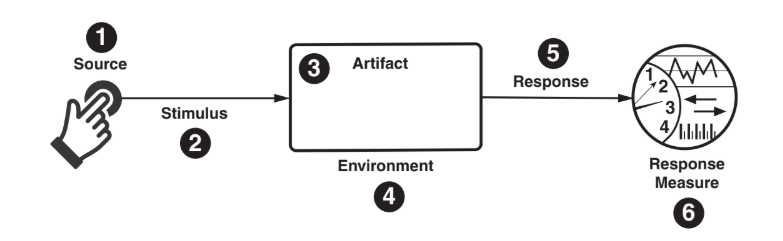
\includegraphics[width=\linewidth]{images/qa_scenario.png}
  \caption{Quality attribute scenario template}
  \caption*{Source: Software Architecture in Practice, 4th edition \cite{bass2021software}}
  \label{fig:qa_scenario_template}
\end{figure}

According to our requirements described in section \ref{sec:problem}, the two main QAs in focus are Availability and Integrability.

\subsection{Availability scenario 1}

\subsubsection{Source}
HMI is running

\subsubsection{Stimulus}
HMI crashes due to a runtime error

\subsubsection{Artifact}
HMI software

\subsubsection{Environment}
Normal operation

\subsubsection{Response}
HMI software is automatically restarted

\subsubsection{Response Measure}
Maximum downtime is 1 second

\begin{figure}[h]
\centering
  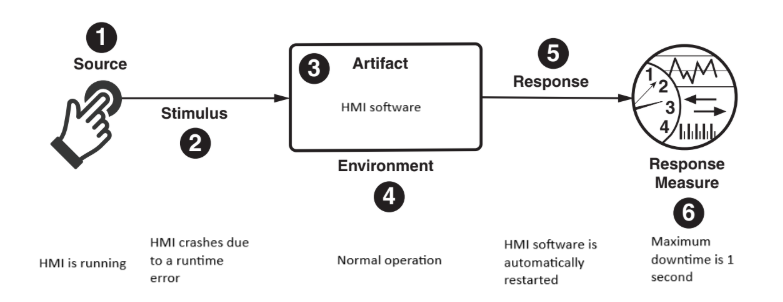
\includegraphics[height=3cm]{images/qa_scenario_hmi_downtime.png}
  \caption{Availability scenario 1}
  \caption*{Source: Software Architecture in Practice, 4th edition \cite{bass2021software}}
  \label{fig:qa_availability_scenario_1}
\end{figure}

\subsection{Availability scenario 2}

\subsubsection{Source}
Production line is running with multiple AGC instances as replicas

\subsubsection{Stimulus}
One of the AGC instances crashes

\subsubsection{Artifact}
AGC software

\subsubsection{Environment}
Normal operation

\subsubsection{Response}
The remaining AGCs continue working

\subsubsection{Response Measure}
No downtime

\begin{figure}[h]
\centering
  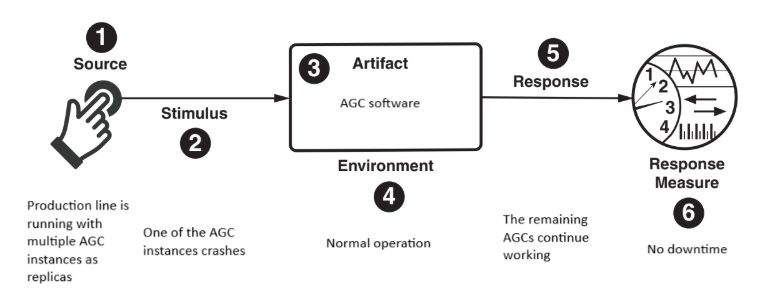
\includegraphics[height=3cm]{images/qa_scenario_agc_downtime.png}
  \caption{Availability scenario 2}
  \caption*{Source: Software Architecture in Practice, 4th edition \cite{bass2021software}}
  \label{fig:qa_availability_scenario_2}
\end{figure}

\subsection{Integrability scenario 1}

\subsubsection{Source}
Production line

\subsubsection{Stimulus}
New AGC instance is ready to add to the production line

\subsubsection{Artifact}
System

\subsubsection{Environment}
Production

\subsubsection{Response}
The new AGC is added and ready to use

\subsubsection{Response Measure}
Maximum 24 hours with no more than 24 person hours of effort
\begin{figure}[h]
\centering
  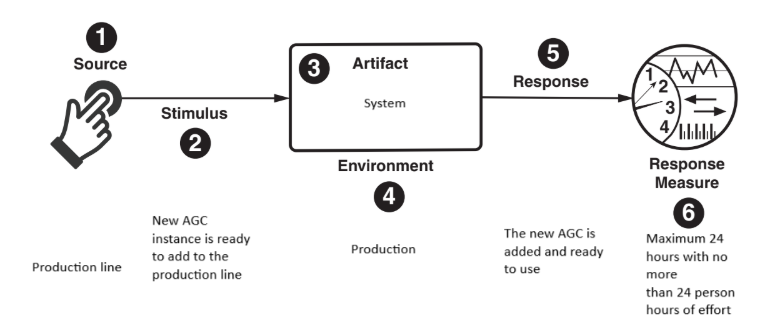
\includegraphics[height=3cm]{images/qa_scenario_deploy_new_agc.png}
  \caption{Integrability scenario 1}
  \caption*{Source: Software Architecture in Practice, 4th edition \cite{bass2021software}}
  \label{fig:qa_integrability_scenario_1}
\end{figure}

% Description of the overall architecture designs
% Argue for tactics used to archieve the QASes
% Discuss the trade-offs

%The architecture needs to support some important scenarios. The production software must run 24/7 which means that production should be able to start at any time. The production line is expected to run 7 hours a day 5 days a week on average and the product can be changed at any time, even multiple times a day. In addition to these, since the company expects a huge growth in a short period of time, the architecture should be designed in a way that new components may easily be added to the production line. Regarding these scenarios, the two main QAs in focus are Availability and Integrability.

\section{Quality Attribute Scenario}
\label{sec:qas}
In this section we are going to discuss quality attribute scenarios. Quality attribute scenario is a common form to describe requirements related to quality attributes. It consists of six parts: Source, Stimulus, Artifact, Environment, Response, and Response Measure.
\begin{enumerate}
    \item (Stimulus) Source: This describes where the stimulus comes from. E.g. a user generated a stimulus by logging into the system or clicking a button.
    \item Stimulus: Description of an event arriving at the system.
    \item Artifact: This is where the Stimulus arrives at. Might be the whole system or any smaller part of the whole system.
    \item Environment: Environment is the combination of factors and conditions that influence a situation. In other words, it is a set of circumstances for the scenario. The environment sets the context for the scenario.
    \item Response: This is the activity that happens when a stimulus has arrived.
    \item Response Measure: The Response should be measurable in some way which makes it testable. The Response Measure describes how the scenario can be tested, so it is decidable whether the architect solved the specific requirement for the system.
\end{enumerate}
We use the template below to illustrate a quality attribute scenario \ref{fig:qa_scenario_template}
\begin{figure}[h]
\centering
  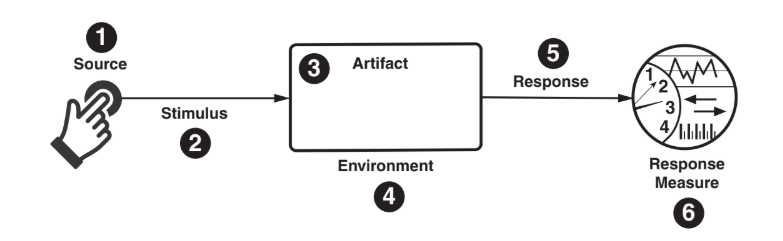
\includegraphics[width=\linewidth]{images/qa_scenario.png}
  \caption{Quality attribute scenario template}
  \caption*{Source: Software Architecture in Practice, 4th edition \cite{bass2021software}}
  \label{fig:qa_scenario_template}
\end{figure}

According to our requirements described in section \ref{sec:problem}, the two main QAs in focus are Availability and Integrability.

\subsection{Availability scenario 1}

\subsubsection{Source}
HMI is running

\subsubsection{Stimulus}
HMI crashes due to a runtime error

\subsubsection{Artifact}
HMI software

\subsubsection{Environment}
Normal operation

\subsubsection{Response}
HMI software is automatically restarted

\subsubsection{Response Measure}
Maximum downtime is 1 second

\begin{figure}[h]
\centering
  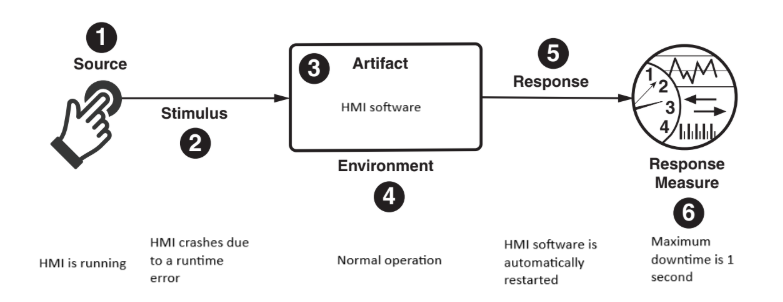
\includegraphics[height=3cm]{images/qa_scenario_hmi_downtime.png}
  \caption{Availability scenario 1}
  \caption*{Source: Software Architecture in Practice, 4th edition \cite{bass2021software}}
  \label{fig:qa_availability_scenario_1}
\end{figure}

\subsection{Availability scenario 2}

\subsubsection{Source}
Production line is running with multiple AGC instances as replicas

\subsubsection{Stimulus}
One of the AGC instances crashes

\subsubsection{Artifact}
AGC software

\subsubsection{Environment}
Normal operation

\subsubsection{Response}
The remaining AGCs continue working

\subsubsection{Response Measure}
No downtime

\begin{figure}[h]
\centering
  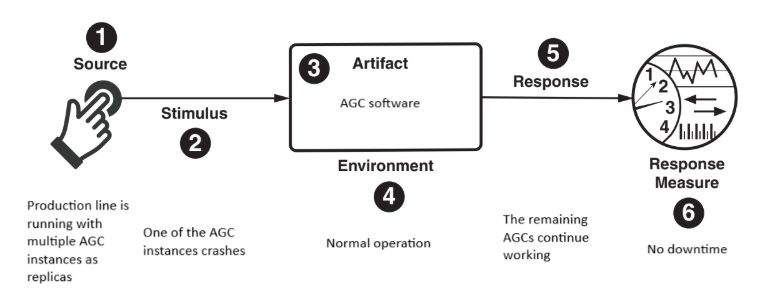
\includegraphics[height=3cm]{images/qa_scenario_agc_downtime.png}
  \caption{Availability scenario 2}
  \caption*{Source: Software Architecture in Practice, 4th edition \cite{bass2021software}}
  \label{fig:qa_availability_scenario_2}
\end{figure}

\subsection{Integrability scenario 1}

\subsubsection{Source}
Production line

\subsubsection{Stimulus}
New AGC instance is ready to add to the production line

\subsubsection{Artifact}
System

\subsubsection{Environment}
Production

\subsubsection{Response}
The new AGC is added and ready to use

\subsubsection{Response Measure}
Maximum 24 hours with no more than 24 person hours of effort
\begin{figure}[h]
\centering
  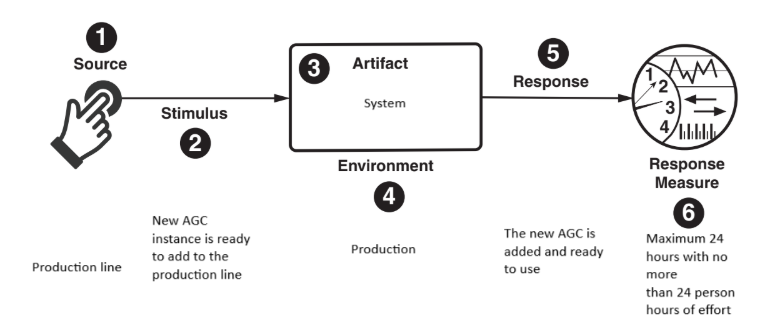
\includegraphics[height=3cm]{images/qa_scenario_deploy_new_agc.png}
  \caption{Integrability scenario 1}
  \caption*{Source: Software Architecture in Practice, 4th edition \cite{bass2021software}}
  \label{fig:qa_integrability_scenario_1}
\end{figure}

% Description of the overall architecture designs
% Argue for tactics used to archieve the QASes
% Discuss the trade-offs

%The architecture needs to support some important scenarios. The production software must run 24/7 which means that production should be able to start at any time. The production line is expected to run 7 hours a day 5 days a week on average and the product can be changed at any time, even multiple times a day. In addition to these, since the company expects a huge growth in a short period of time, the architecture should be designed in a way that new components may easily be added to the production line. Regarding these scenarios, the two main QAs in focus are Availability and Integrability.

\section{Design and Analysis Modeling}
\label{sec:design_and_analysis_modelling}
We have four main systems, such as production management system, supply chain management system, communication management system, and availability management system. But among them, we are focusing only on the production management system and its features. There are multiple ways to represent software architectures, which can be seen in \ref{SysMLDiagram}. The proposed system for the architecture is illustrated in \ref{Featuremodel}. In this system, we have a production control system and a monitoring system where the first one contains operation and inventory features and the last one have logging and operational status features.

\begin{figure}[h]
\centering
  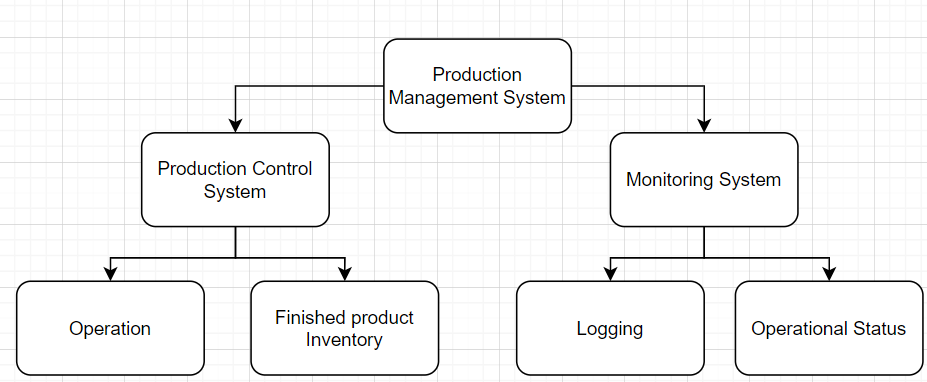
\includegraphics[width=\linewidth]{images/featuremodel.png}
  \caption{Feature model of the system}
  \label{Featuremodel}
\end{figure}

If we explore deep inside our block definition diagram (BDD), we have three main components \ref{fig:boat1}. They are Human Machine Interface (HMI), communication middleware (Bus), and automated guided cart (AGC). To support those components, we have a database component for logging the events. The main function of our HMI is to orchestrate stimulus from the environment and translate those signals through the functional block “Controller” for various purposes. For example, in our use case one, the production manager wants to start operation, so he interacts with the HMI through a start button and the controller generates a message to publish this information to the bus and the AGC, which is subscribed to this bus, receives the data, logs an acknowledgment to the database, and simultaneously initiates its operation for the production. 

\begin{figure}[h]
\centering
  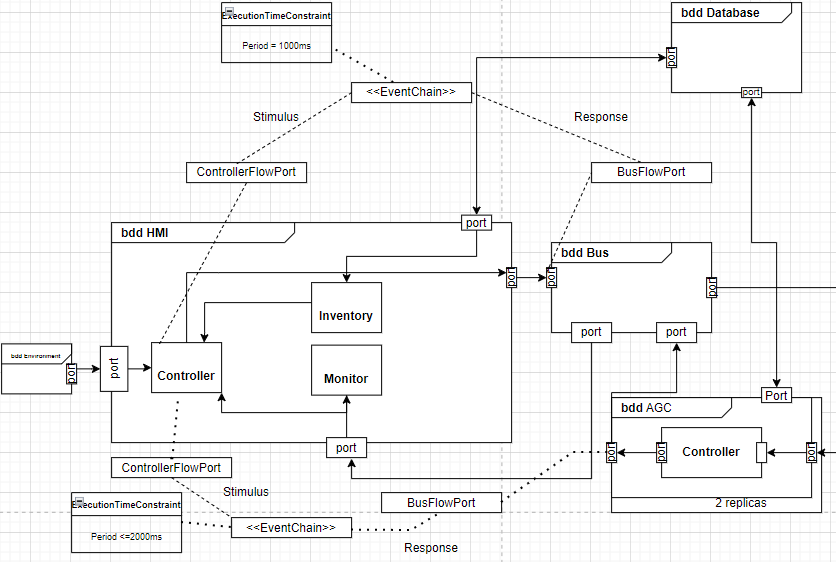
\includegraphics[width=\linewidth]{images/structuremodel2.png}
  \caption{Structure of the system}
  \label{fig:boat1}
\end{figure}

There are different programming languages that have their own merits and advantages for various developments. We select two different programming languages for our two software interacting interfaces. For HMI, we are going with next.js as it is full-stack and it has a clear advantage to make UI components using react.js as well as a backend feature. On the other hand, for the AGC, a lightweight and integrable programming language was highly desirable. Python has all of those qualities, as well as easy syntax with a strong community. Although performance might be a hindrance, we trade off this quality with others. When we are selecting our database for our logging and inventory management, we are looking for ACID compliant (Atomicity, Consistency, Isolation, Durability) and PostgreSQL is perfect for this as it also ensures data integrity and reliability, which can be critical for an inventory tracking system. For choosing the message bus, there was a lot of different benefits between Apache Kafka, pure MQTT, RabbitMQ and more. In the end we selected RabbitMQ as it has both AMQP and MQTT features, and it is lightweight with compared to Apache Kafka.

\begin{table}[h]
\begin{tabular}{|p{1cm}|p{7cm}|}
\hline
ID & Description \\
\hline
Req\#1 & The system will provide a button for the production manager(user) where the manager will start production, the HMI will take this as an action for producing signals to other components to start working. \\
\hline
Req\#2 & The HMI controller will generate a message for publication. \\
\hline
Req\#3 & The HMI controller will publish the generated message to the BUS system which transmits this message to all components in less than 1 second. \\
\hline
Req\#3.1 & Log the operation’s information for the product into the database. \\
\hline
Req\#4 & The AGC component will receive the message from HMI controller within 2 Sec. \\
\hline
Req\#4.1 & Log the operation’s receiving information for the product into database. \\
\hline
Req\#5 & After receiving the "start production" message, AGC will start its production. \\
\hline
Req\#6 & After completing a task, AGC will publish a message indicating it has finished. \\
\hline
Req\#6.1 & Log AGC task completion of the production into the database. \\
\hline
Req\#7 & HMI will receive the quantity of the product and completes the production. \\
\hline
\end{tabular}
\caption{Requirement table}
\label{tab:req_table}
\end{table}

According to our top-level requirements \ref{tab:req_table}, we have emphasized our attention in two main quality attributes (QAs), one is availability and the other are integrability. There are certain points behind these QAs. Availability refers to the system's uptime for its core functionality all the time and it builds on the concept that whenever a system is down it will recover itself through different means as it seems it masks the faults as if it never happened. It is closely related to performance but differs when the system has failed, as the system will still be available but might respond more slowly. It is also closely related to safety as it prevents a system from entering a hazardous state or limiting damage when it does, and lastly closely but clearly distinct from security\cite{bass2021software}. For achieving availability we use the active redundancy pattern and Docker, which helps us to achieve this as it ensures if any faults occur then Docker will use redundant spare. The benefit of this pattern is that it requires a brief delay in the presence of a failure where the alternative would require the system to stop and repair it which would take hours or days. The downside of its cost and complexity. 

We chose integrability as our other QA keeping in mind that we need to integrate different components in our system and use a communication bus. We prefer to decouple our components so that we could add more components with different types more easily and without any dependency. However, to achieve this quality we have to tradeoff performance but it could help us modify it more easily which is our future plan. For achieving this QA, we use orchestration tactics as our HMI is the main coordinator. It collects information and publishes and receives information from other components like AGC through our message bus RabbitMQ. One of the main problems of this tactic is if our bus system is crushed then the whole system will break down, and to overcome this we use Docker containers for our bus with replication. 

\section{Formal verification and validation}
\label{sec:formal_v_and_v}
Formal verification uses mathematical concepts to determine if a system satisfies requirements and operates as intended in all scenarios. Formal verification provides a high degree of assurance that the technology or system will function dependably in all circumstances, in contrast to routine testing, which examines particular scenarios. 

The proposed production system must undergo rigorous verification and validation  to guarantee its stability and reliability. With an emphasis on vital quality features like availability and integrity, this section describes the methodology for comparing the system's behavior to the main criteria.\cite{formalverification}

To evaluate our software system, we must test if the specified requirements are satisfied. The reason for conducting formal verification at this point of the project was to verify and mitigate potential errors made in the design level of the product line. This can save a lot of development time since errors identified earlier can be fixed much easier rather than identifying them in the later phases of the project.

UPPAAL is an effective tool for employing timed automata to describe, simulate, and validate the functioning of real-time systems. It is perfect for verifying systems where schedule and dependability is crucial since it enables users to examine system characteristics like fault tolerance and timing limitations. Using temporal logic specifications, we use UPPAAL to evaluate and validate the system model against these criteria, and ensure that the system fulfills properties such as liveness, safety and avoids deadlocks.\cite{Uppaal} An example of a timed automata can be seen in \ref{fig:TimedAutomata}


 %A. Verification Goals
%The following are the main objectives of the verification process:
%1. Ensure System Resilience: The system should be able cope with errors, including component fails, with little interruption, allowing it to continue operating.

%. Support Dynamic Scaling: Within the time frame and effort limits, the system should make it easier to integrate new AGC instances.

The three figures \ref{fig:Productline} represents the production line in UPPAAL. It's split into the user, who has two options of interaction with the system, namely starting production and requesting a database lookup, our HMI and a model of the AGC which subscribes the message bus. This model allows 
\begin{figure}[h]
  \centering
  \begin{subfigure}[b]{0.4\linewidth}
    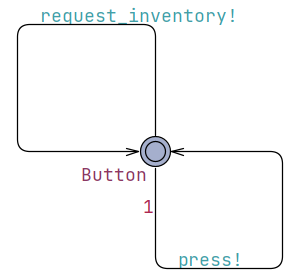
\includegraphics[width=\linewidth]{images/User.png}
     \caption{User}
  \end{subfigure}
  \begin{subfigure}[b]{0.5\linewidth}
    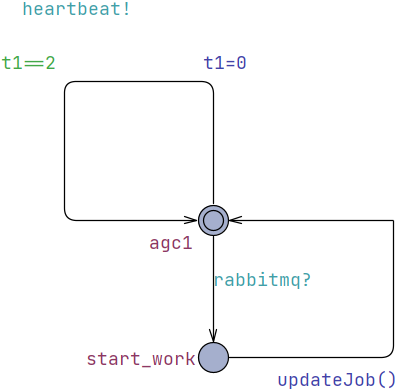
\includegraphics[width=\linewidth]{images/AGC.png}
    \caption{AGC}
  \end{subfigure}
  \begin{subfigure}[b]{0.7\linewidth}
    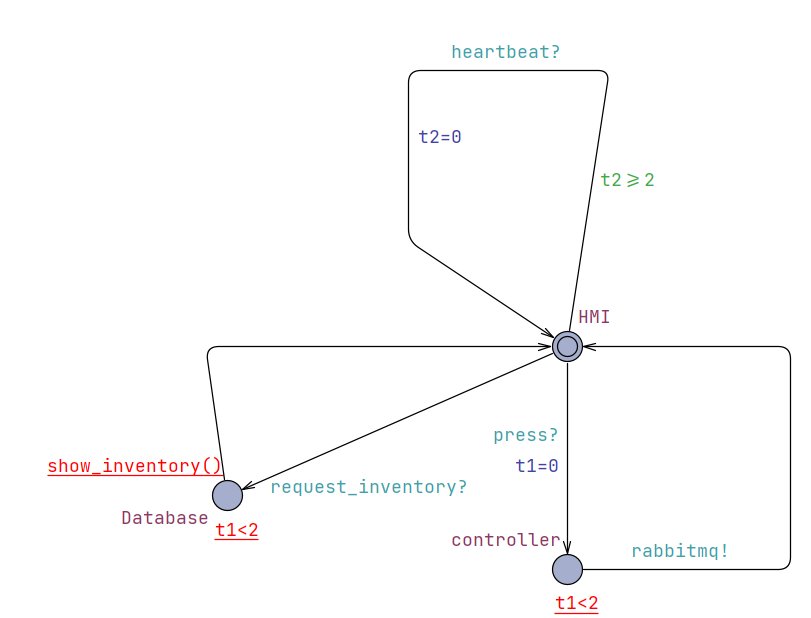
\includegraphics[width=\linewidth]{images/HMI.png}
    \caption{HMI}
  \end{subfigure}
  \caption{Formal verification model of production line}
  \label{fig:Productline}
\end{figure}




\ref{fig:Productline} is a specification of the vital parts of the product line system which can be formally verified. Most of the queries that are verified are directly corresponding to the requirements specified in \ref{tab:uppaal_queries} as seen by their id. The first query to be verified ensures that there are no deadlocks occurring in our behavioral model of the Product line. The second query from the Controller of the HMI to the AGC is a query that verifies the liveness of our system guaranteeing that, starting from the Controller state, the system will eventually reach AGC.start\_work which is the state in which the service subscribed to the message bus has received the signal to start production. This query corresponds to req\#5 from the previous section. The third query verifies that the AGC service, from receiving a message, will eventually reach back to the initial state agc1, meaning that the job has finished. The fourth query which checks for liveness between the AGC receiving the order, to finishing it, was not verifiable. The remaining queries ensure that all the states vital are reachable, and eventually return to the initial state where all actions start from. 


\begin{table}[h]
\centering
\begin{tabular}{|p{4.5cm}|c|c|}
\hline
Query & Status & ReqId \\ \hline
A[] not deadlock & Verified & Req\#1 \\ \hline
$HMI.controller \rightarrow $AGC.start\_work & Verified &  Req\#5 \\ \hline
$A<> $AGC.start\_work and $jobsStart>=$1 imply AGC.agc1 & Verified & - \\ \hline
$AGC.start\_work \rightarrow $AGC.agc1   & Not Verified  & - \\ \hline
$E<> $HMI.Database  & Verified & Req\#4.1 \\ \hline
$HMI.controller \rightarrow $HMI.HMI & Verified  &Req\#6 \\ \hline
$HMI.Database \rightarrow $HMI.HMI & Verified & Req\#6.1 \\ \hline
\end{tabular}
\caption{UPPAAL queries}
\label{tab:uppaal_queries}
\end{table}

\section{Evaluation}
\label{sec:evaluation}

% Empirical evaluation
In this section we are discussing how we conducted the evaluation of our architecture. It consists of four parts: experiment design where we describe the design of the experiment to evaluate the system, measurements where we describe the measurements we made to evaluate the system, pilot test where we describe and computes the number of replications in the actual evaluation and analysis where we present the results from the experiment. We conducted two different experiments on two quality attribute scenarios: Availability scenario 1 and Availability scenario 2. We conducted both experiments in a Dockerized environment.

\subsection{Experiment design}
\label{sec:design}
Before we design our experiment, we need to understand some key concepts for the experiment process. One of the key concepts are the experiment principles. The experiment principles can be seen in the figure below \ref{fig:experiment_principles}.

\begin{figure}[ht]
\centering
  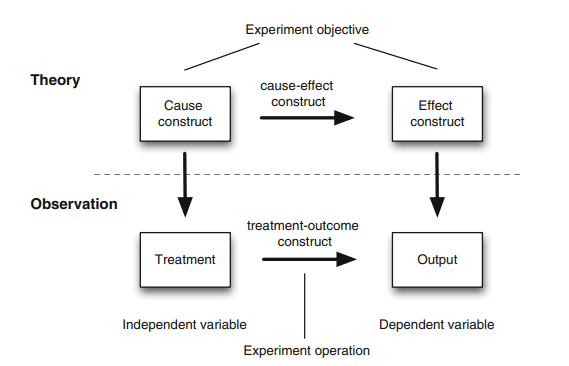
\includegraphics[width=\linewidth]{images/experiment_principles.png}
  \caption{Experiment principles}
  \caption*{Source: Experimentation in Software Engineering}
  \cite{experimentationInSoftwareEngineering}
  \label{fig:experiment_principles}
\end{figure}

This figure shows the theory level and the observation level of an experiment. Theory means that we think that there is some relationship between cause construct and the effect construct. Based on this theory we can construct a hypothesis. On the observation level we test this hypothesis. After the experiment is performed, we are able to observe the results. On the observation level we have some variables, we can consider them "input" variables which are also called independent variables and then we do a treatment on one of those independent variables while trying to fix the levels of other independent variables to make sure they do not modify the result of the experiment. Using this flow, we can observe how the treatment modifies the dependent variable. The illustration of an experiment can be seen in the figure below \ref{fig:experiment_illustration}.

\begin{figure}[ht]
\centering
  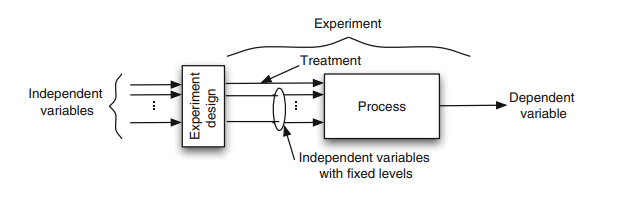
\includegraphics[width=\linewidth]{images/experiment_illustration.png}
  \caption{Illustration of an experiment}
  \caption*{Source: Experimentation in Software Engineering}
  \cite{experimentationInSoftwareEngineering}
  \label{fig:experiment_illustration}
\end{figure}

In our case, we run the experiments in a Dockerized environment to make sure that those independent variables we do not want to do treatment on are fixed.

\subsubsection{Experiment 1}
\label{sec:experiment_1}
In our first experiment we would like to measure how much does it take for a message to reach the AGC from publishing it by the HMI. In our architecture AGC is replicated, which means that we have multiple AGC instances running in parallel. For our experiment we have exactly two AGC instances running. And we do the following treatment: we stop one of the AGC instances for 10 seconds and then we restart it and let it run for 10 seconds, and then stop again for 10 seconds. And we do this as long as we are conducting the experiment. Our hypothesis is that the actual number of AGC instances running does not affect the amount of time needed for the message to reach the AGC.

\subsubsection{Experiment 2}
\label{sec:experiment_2}
In the second experiment we would like to measure how long it takes for the HMI software, which runs in a Docker container, to restart after an unexpected crash. HMI software is designed to be immediately restarted after a crash happens. The treatment here is that we simulate a crash in the HMI software and then measure how much time it takes for the HMI to be up and running again. Our hypothesis is that it should be up in less than 1 second.

\subsection{Measurements}
\label{sec:measurements}
\subsubsection{Experiment 1}
In the case of the first experiment we started the timer when the Start production button was pressed on the HMI screen and stopped the timer when the AGC received the message.

\subsubsection{Experiment 2}
In the case of our second experiment we start the timer when the HMI software started the boot up process and stop the timer when HMI software became fully functional.

\subsection{Pilot test}
\label{sec:pilot_test}
In this section, we are presenting the results we received from the experiments. We only show the first 10 measurements here, but in the scatter plot we display all the measurements we made for both experiments.

\subsubsection{Experiment 1}
After running the first experiment we received the following results: \ref{tab:experiment_1_results}

\begin{table}[ht]
    \centering
    \begin{tabular}{ccc}
       \textbf{ID} & \textbf{Elapsed Time (ms)} & \textbf{Ack.} \\ \hline
       1 & 74 & Success \\
       2 & 43 & Success \\
       3 & 39 & Success \\
       4 & 53 & Success \\
       5 & 66 & Success \\
       6 & 41 & Success \\
       7 & 48 & Success \\
       8 & 53 & Success \\
       9 & 41 & Success \\
       10 & 58 & Success \\
       ... & ... & ... \\
    \hline
    \end{tabular}
    \caption{Measurements for Experiment 1 \ref{sec:experiment_1}}
    \label{tab:experiment_1_results}
\end{table}

\subsubsection{Experiment 2}
We got the following results from the second experiment: \ref{tab:experiment_2_results}
\begin{table}[ht]
    \centering
    \begin{tabular}{cc}
       \textbf{ID} & \textbf{Elapsed Time (ms)} \\ \hline
       1 & 77 \\
       2 & 77 \\
       3 & 82 \\
       4 & 78 \\
       5 & 81 \\
       6 & 79 \\
       7 & 80 \\
       8 & 82 \\
       9 & 101 \\
       10 & 81 \\
       ... & ... \\
    \hline
    \end{tabular}
    \caption{Measurements for Experiment 2 \ref{sec:experiment_2}}
    \label{tab:experiment_2_results}
\end{table}

\subsection{Analysis}
\label{sec:analysis}
In this section we do the analysis on the results we got after running the experiments. For each experiment, we created a scatter plot on which the elapsed time and the ordinal is shown. After that, we calculated the average elapsed time for both experiments.

\subsubsection{Experiment 1}
For the first experiment we did 44 measurements, and we made a scatter plot to show all the measurements and the elapsed time.


\begin{figure}[ht]
\centering
  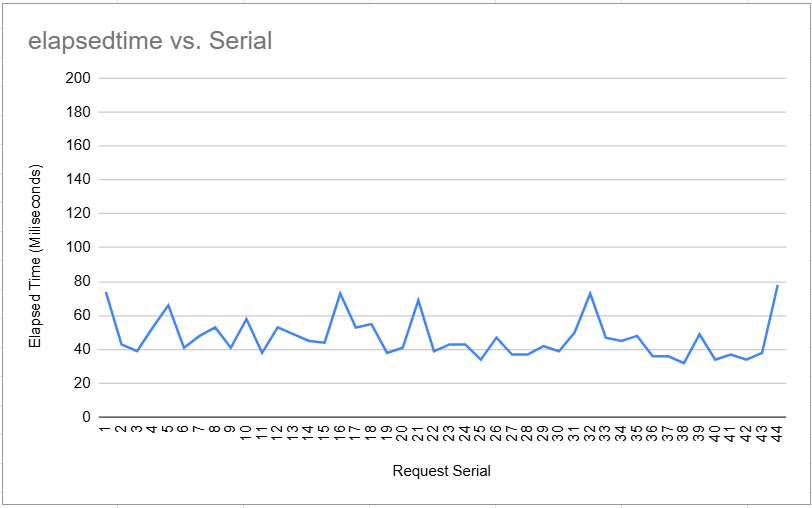
\includegraphics[height=5cm]{images/experiment_1_plot.png}
  \caption{Scatter plot of the first experiment}
  \label{fig:experiment_1_plot}
\end{figure}


In this scatter plot \ref{fig:experiment_1_plot}, it is visible that the Elapsed Time is between 70 and 100 ms. The average Elapsed Time is 47.1 ms. Based on these numbers we can say that the Elapsed Time is not dependent on how many AGC instances are running, which means there is no downtime.
\subsubsection{Experiment 2}
For the second experiment we also did 44 measurements. The figure below shows the scatter plot for the second measurement.

\begin{figure}[ht]
\centering
  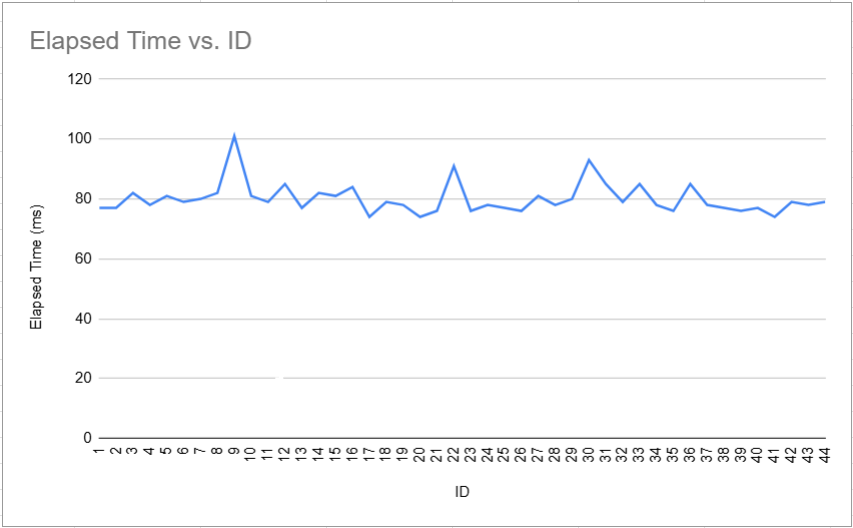
\includegraphics[height=5cm]{images/experiment_2_plot.png}
  \caption{Scatter plot of the first experiment}
  \label{fig:experiment_2_plot}
\end{figure}

In the case of the second experiment the Elapsed Time is between 70 and 100 ms, and their average is 80.1 ms which is significantly less than 1 second stated in our requirements.
\section{Conclusion}
\label{sec:conclusion}
%Conclusion of the report, discussion and relevant future work.

\subsection{Discussion}
\label{sec:Discussion}
%Summary of the work and result(from slides)
%- Discuss our architecture and initial problem/requirements and compare it to the result.(what do we think about it now?) 
The aim of this paper was to solve the obstacles that the pharmaceutical company was facing in order to grow its business and manufacturing capabilities. This came from a list of requirements from this company, (1) as seen in \ref{sec:problem}. Three research questions were then defined from these requirements, (1) How can different architectures support the stated production system requirements?(2) Which architectural trade offs must be taken due to the technology choices? (3) Which properties can be modeled, validated, and verified, and what are the results? The proposition we came up with was the software architecture seen in two levels \ref{Featuremodel} and \ref{fig:boat1}. These models were made as a prototype of the proposed architecture due to time constraints and the scope of our project. The most vital part was modeled here and implemented to facilitate the chosen quality attributes in our system, namely availability and integrity. The proposed design we chose ensured more availability and integrity by incorporating various tactics from each of the attributes. This led to a trade-off of other attributes and technologies for the system such as performance. The experiment emerging from the design was successful in demonstrating that availability and integrability was incorporated into the architecture. The results from both the formal verification and the experiment were satisfactory as they both fulfilled the requirement defined in \ref{tab:req_table}. By containerizing the each component of the system, scalability capabilities has increased heavily also, as Additional services can be added to the container and split the workload.  


%- Discuss our approach to the problem?(usercase - qa- formal verification - implementation - experiment)
%- Discuss the validity of our experiment(how did this?)

\subsection{Future work}
\label{sec:future_work}
%Discuss how the work can be extended with respect to the approach and/or evaluation(from slides) 

In our architecture, we are concentrated on availability and integrability options, and here we have a common communication bus to fulfill our message transportation between components. But there is a problem if this bus fails, there is no alternative, which will be our future work as well as we will also intend to incorporate the deployability quality attribute into the software architecture, so that the system could be more efficiently deployable. For availability, we would like to focus more on how the system could detect the fault before it could happen, and if we have faults, it could roll back to the previous workable state so that there will be no effect for the consumers. 
%%% Conclusion



\bibliographystyle{IEEEtran}
\bibliography{references}
\begin{appendices}
\section{Appendices}

\begin{figure}[h]
    \centering
    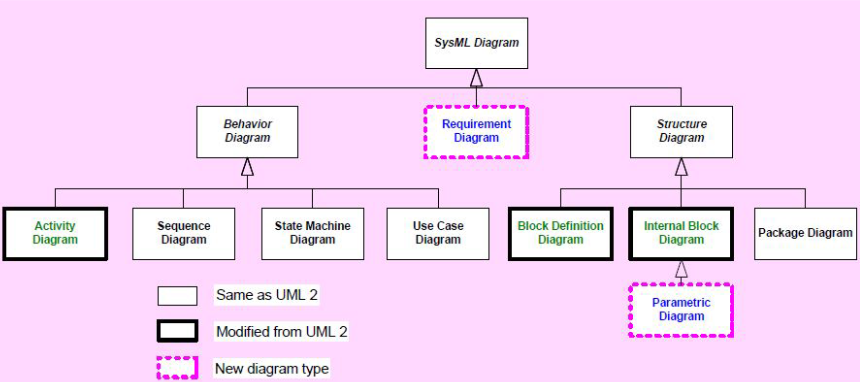
\includegraphics[width=2\linewidth]{images/diagrams.png}
    \caption{SysML Diagram taxonomy \cite{Diagram}}
    \label{SysMLDiagram}
\end{figure}

\pagebreak

\begin{figure}[h]
    \centering
    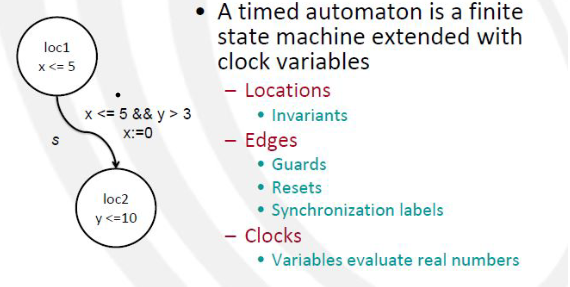
\includegraphics[width=1\linewidth]{images/timedautomata.png}
    \caption{Timed Automata \cite{TimedAutomata}}
    \label{fig:TimedAutomata}
\end{figure}

\end{appendices}
\vspace{12pt}
\end{document}
